\begin{frame}{What is knowledge?}
    \begin{itemize}
        \item
              Are simple facts knowledge?
              \vspace{1em}
              \begin{center}
                  \begin{minipage}{0.7\textwidth}
                      \begin{columns}[c]
                          \column{0.45\linewidth}
                          \centering
                          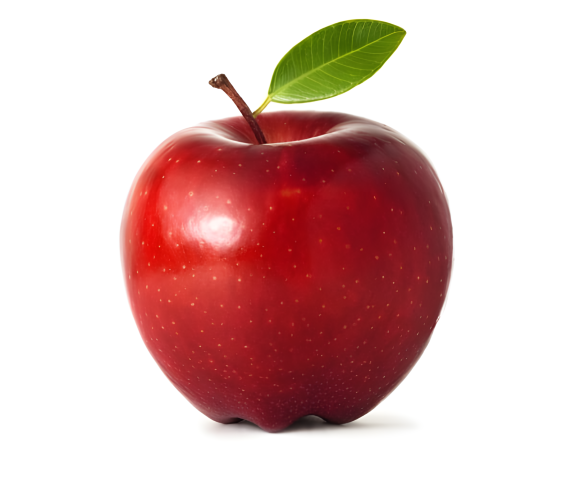
\includegraphics[width=\linewidth]{images/red-apple.png}
                          \captionof{figure}{\gcite{\href{https://www.bodi.com/blog/types-of-apples}{Source}}}
                          %
                          \column{0.1\linewidth}
                          \centering
                          $\xrightarrow{\rule{\linewidth}{0pt}}$
                          \column{0.45\linewidth}
                          This apple is red.
                      \end{columns}
                  \end{minipage}
              \end{center}
        \item \bhighlight{Logical atomism} is the view that reality consists of simple, independent facts (“atomic facts”) and that complex statements can be analyzed into combinations of these basic facts.
    \end{itemize}
\end{frame}

\begin{frame}{What is knowledge?}
    \begin{itemize}
        \item
              Is it the ability to predict interactions and events?
              \vspace{1em}
              \begin{center}
                  \begin{minipage}{0.7\textwidth}
                      \begin{columns}[c]
                          \column{0.45\linewidth}
                          \centering
                          Apples fall downward when dropped from a tree.
                          \column{0.1\linewidth}
                          \centering
                          $\xrightarrow{\rule{\linewidth}{0pt}}$
                          \column{0.45\linewidth}
                          \centering
                          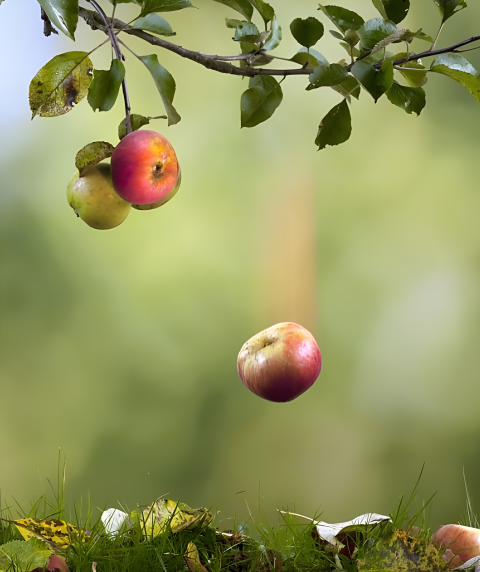
\includegraphics[width=\linewidth]{images/apple-falling.png}
                          \captionof{figure}{\gcite{\href{https://uk.pinterest.com/pin/prints-of-picture-no-10946968--794955771754853849/}{Source}}}
                      \end{columns}
                  \end{minipage}
              \end{center}
        \item \bhighlight{Instrumentalism} holds that the primary value of a theory or proposition is its \bhighlight{predictive} (and practical) efficacy—even if it doesn't claim to mirror some deeper reality.
    \end{itemize}
\end{frame}

\begin{frame}{What is knowledge?}
    \begin{itemize}
        \item
              Is ``verifiability'' important?
              \vspace{1em}
              \begin{center}
                  \begin{minipage}{0.7\textwidth}
                      \begin{columns}[c]
                          \column{0.45\linewidth}
                          Somewhere in the universe, there exists an apple that will ``fall'' upwards if no one is around to check.
                          \column{0.10\linewidth}
                          \centering
                          $\xleftrightarrow{\hspace*{0.5\linewidth}?\hspace*{0.5\linewidth}}$
                          \column{0.45\linewidth}
                          \centering
                          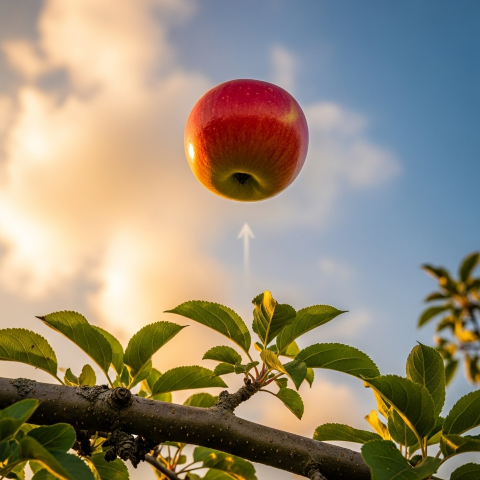
\includegraphics[width=\linewidth]{images/apple-rising.png}
                          \captionof{figure}{\gcite{\href{https://deepmind.google/models/imagen/}{Source}}}
                      \end{columns}
                  \end{minipage}
              \end{center}
        \item \bhighlight{Logical empiricism} expands on \bhighlight{logical atomism} to add a \bhighlight{verifiability} constraint. In order for a proposition to be meaningful,
              it needs to be verifiable, even if only in theory.
    \end{itemize}
\end{frame}